\documentclass[a4paper,12pt]{article}

\usepackage[T2A]{fontenc}			
\usepackage[utf8]{inputenc}			
\usepackage[english,russian]{babel}	

\usepackage[
bookmarks=true, colorlinks=true, unicode=true,
urlcolor=black,linkcolor=black, anchorcolor=black,
citecolor=black, menucolor=black, filecolor=black,
]{hyperref}

\usepackage{color}
\usepackage{caption}
\DeclareCaptionFont{white}{\color{black}}
\DeclareCaptionFormat{listing}{\colorbox{white}{\parbox{\textwidth}{#1#2#3}}}
\captionsetup[lstlisting]{format=listing,labelfont=white,textfont=white}

\usepackage{amsmath,amsfonts,amssymb,amsthm,mathtools} 
\usepackage{wasysym}

\usepackage{graphicx}
%\usepackage[cache=false]{minted}
\usepackage{cmap}
\usepackage{indentfirst}

\usepackage{listings} 
\usepackage{fancyvrb}

\usepackage{geometry}
\geometry{left=2cm}
\geometry{right=1.5cm}
\geometry{top=1cm}
\geometry{bottom=2cm}

\setlength{\parindent}{5ex}
\setlength{\parskip}{0.5em}

\begin{document}
\lstset{ %
	language=C++,                 % выбор языка для подсветки (здесь это С)
	basicstyle=\small\sffamily, % размер и начертание шрифта для подсветки кода
	numbers=left,               % где поставить нумерацию строк (слева\справа)
	numberstyle=\tiny,           % размер шрифта для номеров строк
	stepnumber=1,                   % размер шага между двумя номерами строк
	numbersep=5pt,                % как далеко отстоят номера строк от подсвечиваемого кода
	backgroundcolor=\color{white}, % цвет фона подсветки - используем \usepackage{color}
	showspaces=false,            % показывать или нет пробелы специальными отступами
	showstringspaces=false,      % показывать или нет пробелы в строках
	showtabs=false,             % показывать или нет табуляцию в строках
	frame=single,              % рисовать рамку вокруг кода
	tabsize=2,                 % размер табуляции по умолчанию равен 2 пробелам
	captionpos=t,              % позиция заголовка вверху [t] или внизу [b] 
	breaklines=true,           % автоматически переносить строки (да\нет)
	breakatwhitespace=false, % переносить строки только если есть пробел
	escapeinside={\%*}{*)}   % если нужно добавить комментарии в коде
}


% Титульный лист
\large
\begin{center}
	Федеральное государственное бюджетное образовательное учреждение 
	высшего образования <<Московский государственный технический 
	университет имени Н. Э. Баумана>> 
	(национальный исследовательский университет)
\end{center}

\vspace*{30mm} 


\huge
\begin{center}
	Дисциплина: <<Анализ алгоритмов>>
	
	Отчет по лабораторной работе №5
\end{center}

\vspace*{30mm} 

\huge
\begin{center}
	Тема работы:\\
	<<Конвейерная обработка данных>>
\end{center}
\vspace*{30mm} 

\large
\begin{flushright}
	Студент: Левушкин И. К. \\
	Группа: ИУ7-52Б \\
	Преподаватели: Волкова Л. Л., \\ Строганов Ю. В. \\
\end{flushright}

\vspace*{40mm}
\begin{center}
	Москва, 2019 г.  
\end{center}
\thispagestyle{empty}


\tableofcontents
% \setcounter{page}{1}

\section*{Введение}
\addcontentsline{toc}{section}{Введение}

Имеется большое количество важных задач, решение которых требует использования 
огромных вычислительных мощностей, зачастую недоступных для современных 
вычислительных систем.

Параллелизм может значительно ускорить решение
таких задач. Особое место среди систем подобного рода занимает
конвейерный обработчик. Он прост для понимания,
ведь принцип его работы основан на реальном механизме
непрервного действия. ~\cite{voev}

\textbf{Цель лабораторной работы:} получить навык организации асинхронной передачи 
данных между потоками на примере конвейерной обработки информации

\textbf{Задачи работы:}

\begin{enumerate} 
	\item[1)] изучить алгоритм конвейеризации;
	\item[2)] реализовать конвейерную систему;
	\item[4)] описать и обосновать полученные результаты в отчете о лабораторной 
	работе, выполненного как расчётно-пояснительная записка. 
\end{enumerate} 
\pagebreak

\section{Аналитический раздел}

В данном разделе будет рассмотрен алгоритм конвейеризации.

\subsection{Описание алгоритмов}

\subsubsection{Алгоритм конвейерной обработки данных}

Конвейеризация --- это техника, в результате которой  задача
разбивается  на некоторое число подзадач,
которые  выполняются последовательно.
Конвейерный подход позволяет создавать эффективные параллельные реализации обычных 
неспециализированных алгоритмов. ~\cite{iu7}

Каждая  подкоманда   выполняется на своем логическом  устройстве.
Все     логические    устройства   (ступени)  соединяются последовательно
таким образом, что выход  $i$-ой   ступени   связан   с   
входом   ($i+1$)-ой   ступени,  все ступени  работают  одновременно.  
Множество  ступеней называется    конвейером.    
Выигрыш     во    времени достигается при  выполнении  нескольких задач  
за  счет параллельной   работы   ступеней,  
вовлекая  на  каждом такте новую задачу или команду.  ~\cite{korn}

Каждое звено конвейера выполняет следующие действия:

\begin{itemize}
	\item     получить данные,
	
	\item     обработать данные,
	
	\item      послать данные следующим звеньям.
\end{itemize}

\subsection*{Выводы}
\addcontentsline{toc}{subsection}{Выводы}

Рассмотрен алгоритм конвейерной обработки данных, выделены его ключевые моменты.

\newpage

\section{Конструкторский раздел}

В разделе приводятся схемы выбранных алгоритмов сортировки,
производится их теоретический сравнительный анализ.

\subsection{Разработка алгоритмов}

На рис. \ref{fig:insert} приведена схема 
общая схема конвейерной обработки.

\begin{figure}[h!]
	\begin{center}
		{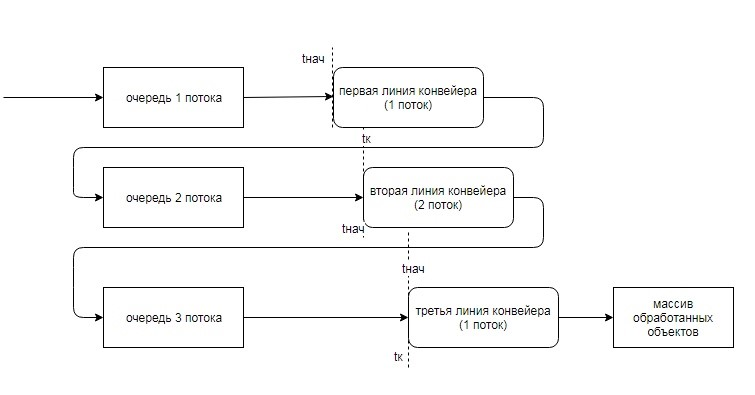
\includegraphics[width=\textwidth]{conv.jpg}}
		\caption{
			Схема работы конвейера}
		\label{fig:insert}
	\end{center}
\end{figure}

Псевдокод главной функции:

\begin{flushleft}
	1. Создать 3 потока, мьютекса и очереди\\
	2. Заполнить массив объектов значениями от 1 до n\\
	3. Добавить элементы массива в очередь 1\\
	4. Применить join ко всем потокам\\
	5. Записать информации из массива результатов в лог-файл\\
\end{flushleft}

Псевдокод для ленты 1:

\begin{flushleft}
	1. Бесконечный цикл\\
		2. \hspace{1.5cm} Заблокировать мьютекс 1\\
		3. \hspace{1.5cm} Если очередь 1 не пуста\\
		4. \hspace{3cm} Извлечь элемент из очереди\\
		5. \hspace{3cm} Записать информацию о начале работы\\
		6. \hspace{3cm} Добавить элемент в результирующий массив\\
		7. \hspace{3cm} Выполнить функции 1\\
		8. \hspace{3cm} Добавить элемент в очередь 2\\
		8. \hspace{3cm} Записать информацию об окончании работы\\
		10. \hspace{3cm} Добавить элемент в результирующий массив\\
		11. \hspace{3cm} Если элемент равен n\\
		12. \hspace{4.5cm} Завершить работу\\
		13. \hspace{1.5cm} Разблокировать мьютекс 1\\
\end{flushleft}

Псевдокод для ленты 2:

\begin{flushleft}
	1. Бесконечный цикл\\
		2. \hspace{1.5cm} Заблокировать мьютекс 2\\
		3. \hspace{1.5cm} Если очередь 2 не пуста\\
		4. \hspace{3cm} Извлечь элемент из очереди\\
		5. \hspace{3cm} Записать информацию о начале работы\\
		6. \hspace{3cm} Добавить элемент в результирующий массив\\
		7. \hspace{3cm} Выполнить функции 2\\
		8. \hspace{3cm} Добавить элемент в очередь 3\\
		9. \hspace{3cm} Записать информацию об окончании работы\\
		10. \hspace{3cm} Добавить элемент в результирующий массив\\
		11. \hspace{3cm} Если элемент равен n\\
		12. \hspace{4.5cm} Завершить работу\\
		13. \hspace{1.5cm} Разблокировать мьютекс 2\\
\end{flushleft}

Псевдокод для ленты 3:

\begin{flushleft}
	1. Бесконечный цикл\\
		2. \hspace{1.5cm} Заблокировать мьютекс 3\\
		3. \hspace{1.5cm} Если очередь 3 не пуста\\
		4. \hspace{3cm} Извлечь элемент из очереди\\
		5. \hspace{3cm} Записать информацию о начале работы\\
		6. \hspace{3cm} Добавить элемент в результирующий массив\\
		7. \hspace{3cm} Выполнить функции 3\\
		8. \hspace{3cm} Записать информацию об окончании работы\\
		9. \hspace{3cm} Добавить элемент в результирующий массив\\
		10. \hspace{3cm} Если элемент равен n\\
		11. \hspace{4.5cm} Завершить работу\\
		12. \hspace{1.5cm} Разблокировать мьютекс 3\\
\end{flushleft}

\subsection*{Выводы}
\addcontentsline{toc}{subsection}{Выводы}

В разделе представлен псевдокод конвейерной обработки данных.
Даны интерпретации главной функции
и 3 функций, имитирующих работу лент.

\newpage

\section{Технологический раздел}

Здесь описываются требования к программному 
обеспечению и средства реализации, приводятся листинги 
программы.

\subsection{Требования к программному обеспечению}

Необходимо реализовать класс object, который будет в себе содержать данные, над которыми будут работать конвейеры и соответственно сами конвейеры (методы класса), которые будут применяться над объектом.

Сами данные объекта будут представлять собой динамический массив, над которым будут совершаться некоторые действия.

В качестве первого конвейера было решено взять сортировку Шелла.
Во втором конвейере происходит добавление 10 * $len(mas)$ элементов к текущему массиву.
И в третьем происходит вывод на экран 1\% всех элементов массива.

\begin{flushleft}
	\textbf{Входные данные:} нет
	
	\textbf{Выходные данные:} 
	\begin{itemize}
		\item номер объекта;
		\item номер конвейера;
		\item время начала выполнения на первом конвейере;
		\item время конца выполнения на первом конвейере;
		\item время начала выполнения на втором конвейере;
		\item время конца выполнения на втором конвейере;
		\item время начала выполнения на третьем конвейере;
		\item время конца выполнения на третьем конвейере;
	\end{itemize}
\end{flushleft}


\subsection{Средства реализации}

Для реализации поставленной задачи был использован язык программирования C++ ~\cite{c}. Проект был выполнен в среде QT Creator ~\cite{qt}. Для измерения процессроного времени была использована ассемблерная инструкция rdtsc ~\cite{rdtsc}.

Для хранения массива, строк применяются 
контейнерные классы \textit{std::vector}, \textit{std::string} из стандартной 
библиотеки шаблонов STL. Кроме того, для реализации конвейера
используются \textit{std::thread} и \textit{std::mutex}.

Замер времени
производится с помощью функции \textit{clock\_gettime} из библиотеки \textit{time.h}.

\subsection{Листинг программы}

Реализованная программа представлена
в листингах \ref{lst0}-\ref{lst4}.

\begin{lstlisting}[label=lst0,caption=Структура класса object]
#include <vector>
#include <iostream>
#include <ctime>

#define DEFAULT_SIZE 10

using namespace std;

struct time_for_work
{
timespec from;
timespec to;
};

class object
{
public:
object();
object(size_t count);
object(vector<int> mas);

void add_elem_to_mas(const int value);

void delete_last_elem_from_mas();

void do_conveyer_1();

void do_conveyer_2();

void do_conveyer_3();

void set_time_1(time_for_work t1) {this->t1 = t1;}
void set_time_2(time_for_work t2) {this->t2 = t2;}
void set_time_3(time_for_work t3) {this->t3 = t3;}

time_for_work get_time_1();
time_for_work get_time_2();
time_for_work get_time_3();

vector<int> get_mas();


~object() = default;

private:
vector<int> mas;
time_for_work t1;
time_for_work t2;
time_for_work t3;
};
\end{lstlisting}

\begin{lstlisting}[label=lst1,caption=Реализация класса object]
#include "object.h"


object::object()
{
this->mas.resize(DEFAULT_SIZE);
for (size_t i = 0; i < this->mas.size(); i++)
{
this->mas[i] = rand();
}
}

object::object(size_t count)
{
this->mas.resize(count);
for (size_t i = 0; i < this->mas.size(); i++)
{
this->mas[i] = rand();
}
}

object::object(vector<int> mas)
{
this->mas = mas;
}

void object::add_elem_to_mas(const int value)
{
this->mas.push_back(value);
}

void object::delete_last_elem_from_mas()
{
this->mas.pop_back();
}

void ShellSort (vector<int>& array)
{
int tmp;
int size = array.size();
for (int step = size / 2; step > 0; step /= 2)
{
for (int i = step; i < size; i++)
{
for (int j = i - step; j >= 0 && array[size_t(j)] > array[size_t(j + step)]; j -= step)
{
tmp = array[size_t(j)];
array[size_t(j)] = array[size_t(j + step)];
array[size_t(j + step)] = tmp;
}
}
}
}

void add_elements(vector<int> &mas)
{
int count_elements = DEFAULT_SIZE * 10;
for (int i = 0; i < count_elements; i++)
{
mas.push_back(rand());
}
}

void print_few_elements(const vector<int> &mas)
{
size_t count_print_elements = mas.size() / 100;
for (size_t i = 0; i < count_print_elements; i++)
{
cout << mas[i] << " ";
if (i % 10 == 0)
{
cout << endl;
}
}
cout << endl;
}

void object::do_conveyer_1()
{
ShellSort(mas);
}

void object::do_conveyer_2()
{
add_elements(mas);
}

void object::do_conveyer_3()
{
print_few_elements(mas);
}

time_for_work object::get_time_1()
{
return t1;
}

time_for_work object::get_time_2()
{
return t2;
}

time_for_work object::get_time_3()
{
return t3;
}

vector<int> object::get_mas()
{
return mas;
}
\end{lstlisting}

\begin{lstlisting}[label=lst2,caption=Лента 1]
void conveyer_1()
{
timespec now, after;
while (1)
{
m1.lock();
if (!q1.empty())
{
auto object = q1.front();
q1.pop();

clock_gettime(CLOCK_REALTIME, &now);
object.do_conveyer_1();
clock_gettime(CLOCK_REALTIME, &after);

object.set_time_1({now, after});

m2.lock();
q2.push(object);
m2.unlock();
counter_1++;
if (counter_1 == count_objects)
{
return;
}
}
m1.unlock();
}
}
\end{lstlisting}

\begin{lstlisting}[label=lst3,caption=Лента 2]
void conveyer_2()
{
timespec now, after;
while (1)
{
m2.lock();
if (!q2.empty())
{
auto object = q2.front();
q2.pop();

clock_gettime(CLOCK_REALTIME, &now);
object.do_conveyer_2();
clock_gettime(CLOCK_REALTIME, &after);

object.set_time_2({now, after});

m3.lock();
q3.push(object);
m3.unlock();
counter_2++;
if (counter_2 == count_objects)
{
return;
}
}
m2.unlock();
}
}
\end{lstlisting}

\begin{lstlisting}[label=lst4,caption=Лента 3]
void conveyer_3(vector<object> &return_objects)
{
timespec now, after;
while (1)
{
m3.lock();
if (!q3.empty())
{
auto object = q3.front();
q3.pop();

clock_gettime(CLOCK_REALTIME, &now);
object.do_conveyer_3();
clock_gettime(CLOCK_REALTIME, &after);


object.set_time_3({now, after});

return_objects.push_back(object);
counter_3++;
if (counter_3 == count_objects)
{
return;
}
}
m3.unlock();
}
}
\end{lstlisting}

\begin{lstlisting}[label=lst5,caption=main]
mutex m1, m2, m3;
queue<object> q1, q2, q3;
size_t count_objects = 100;
size_t counter_1 = 0;
size_t counter_2 = 0;
size_t counter_3 = 0;

vector<object> objects_generator(size_t count_objects)
{
vector<object> mas_objects;
for (size_t i = 0; i < count_objects; i++)
{
object *obj = new object(i * 100);
mas_objects.push_back(*obj);
}
return mas_objects;
}

void print_time(time_for_work tim)
{
long ms_from, ms_to; // Milliseconds
long long ns_from, ns_to; // Nanoseconds
time_t s_from, s_to;  // Seconds
tm *timeinfo_from, *timeinfo_to;

s_from  = tim.from.tv_sec;
timeinfo_from = localtime (&s_from);
ms_from = floor(tim.from.tv_nsec / 1.0e6); // Convert nanoseconds to milliseconds

s_to  = tim.to.tv_sec;
timeinfo_to = localtime (&s_to);
ms_to = floor(tim.to.tv_nsec / 1.0e6); // Convert nanoseconds to milliseconds

ns_from = abs(tim.from.tv_nsec - ms_from * 1.0e6);

ns_to = abs(tim.to.tv_nsec - ms_to * 1.0e6);



cout << "Start: " << timeinfo_from->tm_hour <<
":" << timeinfo_from->tm_min << ":" <<
timeinfo_from->tm_sec << ":" << ms_from << ":" << ns_from << endl;
cout << "Ending: " << timeinfo_to->tm_hour <<
":" << timeinfo_to->tm_min << ":" <<
timeinfo_to->tm_sec << ":" << ms_to << ":" << ns_to << endl;
}

void print_results(vector<object> res)
{
time_for_work tim;

for (size_t i = 0; i < res.size(); i++)
{
cout << "Object " << i << ":" << endl;

cout << "Konveyer 1: " << endl;
tim = res[i].get_time_1();
print_time(tim);

cout << "Konveyer 2: " << endl;
tim = res[i].get_time_2();
print_time(tim);

cout << "Konveyer 3: " << endl;
tim = res[i].get_time_3();
print_time(tim);
}
}

int main()
{
vector<object> mas_objects = objects_generator(count_objects);

vector<object> return_objects;

vector<thread> thr(3);

thr[0] = thread(conveyer_1);
thr[1] = thread(conveyer_2);
thr[2] = thread(conveyer_3, ref(return_objects));

for (size_t i = 0; i < count_objects; i++)
{
q1.push(mas_objects[i]);
}


for (size_t i = 0; i < thr.size(); i++)
{
thr[i].join();
}

print_results(return_objects);

return 0;
}
\end{lstlisting}

\subsection*{Выводы}
\addcontentsline{toc}{subsection}{Выводы}

В данном разделе были рассмотрены требования к 
программному обеспечению, обоснован выбор средств 
реализации, приведены листинги программы.

\newpage

\section{Исследовательский раздел}

В разделе представлены примеры выполнения программы.

\subsection{Примеры работы и анализ файлов журналирования}

На рис. \ref{fig:t0} приведен пример работы программы.
\begin{flushleft}
	\textbf{Обозначения:}\\
	Конвейер № -- номер события,\\
	Начало -- время начала события в формате ч:м:с.мс.нс.\\
	Конец -- время окончания события в формате ч:м:с.мс.нс.
\end{flushleft}

\begin{figure}[h!]
	\center{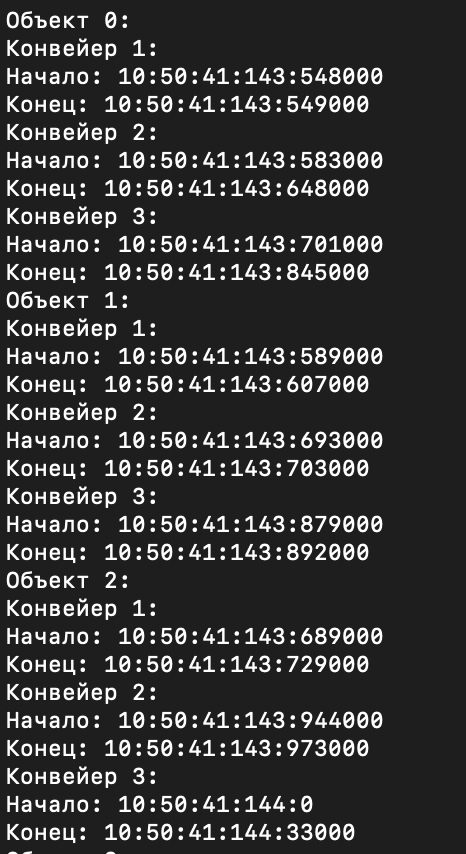
\includegraphics[width=0.5\textwidth]{example2.jpg}}
	\caption{Пример работы программы}
	\label{fig:t0}
\end{figure}


На рисунке можно наблюдать поэтапную обработку
для 3 элементов. Первый объект обслуживается последовательно, то есть вторая и третья ленты ждут пока первая лента обработает первый объект. Затем первая лента начинает обслуживать второй объект в то время как вторая лента начинает обслуживать первый объект и так далее.
Время простоя для каждой ленты
соответствует ожидаемой величине.


\subsection*{Выводы}
\addcontentsline{toc}{subsection}{Выводы}

Программа успешно демонстрирует конвейерную обработку.
Из рисунка можно наблюдать поэтапную обработку для 3 элементов. Время простоя для каждой ленты соответствует ожидаемой величине. Все три ленты работают параллельно, следовательно последовательная обработка будет менее эффективна нежели конвейерная обработка.

\section*{Заключение}
\addcontentsline{toc}{section}{Заключение}

В ходе работы выполнено следующее:

\begin{enumerate} 
	\item[1)] изучен алгоритм конвейеризации;
	\item[2)] реализована конвейерная система;
	\item[4)] описаны и обоснованы полученные результаты в отчете о лабораторной 
	работе, выполненного как расчётно-пояснительная записка. 
\end{enumerate}


\addcontentsline{toc}{section}{Список литературы}
\begin{thebibliography}{10}
	
	\bibitem{mcconell}
	Дж. Макконнелл. Анализ алгоритмов. Активный 
	обучающий 
	подход.-М.:Техносфера, 2009.
	
	\bibitem{knuth}
	Д. Кнут. Искусство программирования, М., Мир, 1978
	
	\bibitem{voev}
	Воеводин В.В. Математические модели и методы в параллельных процессах. М., 1986
	
	\bibitem{iu7}
	Погорелов Д.А. Применение конвейерной обработки данных на примере сортировки простыми вставками, М., Образование и наука в России и за рубежом
	2019 .- Т. 49 , № 1
	
	\bibitem{korn}
	Корнеев В.В. Параллельные вычислительные системы. М., 1999.
	
	\bibitem{std}
	ISO/IEC 14882:2017 [Электронный ресурс]. – Режим доступа: https://www.iso.org/standard/68564.html, свободный – (27.11.2019)
	
	\bibitem{chrono}
	<chrono> [Электронный ресурс]. – Режим доступа: http://www.cplusplus.com/reference/chrono/, свободный – (20.11.2019)
	
	\bibitem{qt} QT Creator Manual [Электронный ресурс]. – Режим
	доступа: https://doc.qt.io/qtcreator/index.html, свободный. (Дата
	обращения: 29.09.2019 г.)
	
	\bibitem{rdtsc} Microsoft «rdtsc» [Электронный ресурс]. – Режим доступа:
	https://docs.microsoft.com/ru-ru/cpp/intrinsics/rdtsc?view=vs-2019,
	свободный. (Дата обращения: 29.09.2019 г.)
	
	\bibitem{c} ISO/IEC JTC1 SC22 WG21 N 3690 «Programming Languages — C++» [Электронный ресурс]. – Режим доступа: https://devdocs.io/cpp/, свободный. (Дата обращения: 29.09.2019 г.)
	
\end{thebibliography}

\end{document}